% ===================================================================
% 半导体电荷存储的物理原理：NAND闪存中的量子隧穿与阈值工程
% ===================================================================

\documentclass[11pt,a4paper,twoside]{article}

% ---------- Encoding & Fonts ----------
\usepackage[UTF8]{ctex}
% CJK fonts auto-detected by ctex (Windows: SimSun/SimHei, macOS: Songti SC/Heiti SC)
\usepackage[T1]{fontenc}
\usepackage{amsthm}
\usepackage{newtxtext,newtxmath}
\usepackage[scaled=0.92]{helvet}
\usepackage{courier}

% ---------- Layout ----------
\usepackage[margin=2.5cm,top=3cm,bottom=2.8cm]{geometry}
\usepackage{setspace}
\onehalfspacing
\usepackage{fancyhdr}
\pagestyle{fancy}
\fancyhf{}
\fancyhead[LE]{\small\itshape 第2篇\quad NAND闪存的物理原理}
\fancyhead[RO]{\small\itshape 量子隧穿与阈值工程}
\fancyfoot[CE,CO]{\thepage}
\renewcommand{\headrulewidth}{0.4pt}

% ---------- Math & Physics ----------
\usepackage{amsmath,amsfonts}
\usepackage{mathtools}
\usepackage{bm}
\usepackage{physics}
\usepackage{siunitx}
\sisetup{separate-uncertainty,per-mode=symbol}
% Custom degree Celsius command (avoids siunitx version issues)


\newcommand{\degC}{\ensuremath{{}^{\circ}\mathrm{C}}}

% ---------- Graphics ----------
\usepackage{graphicx}
\usepackage{xcolor}
\usepackage{tikz}
\usetikzlibrary{arrows.meta,shapes,decorations.pathmorphing,patterns,calc,positioning}
\usepackage{pgfplots}
\pgfplotsset{compat=1.18}
\usepackage{float}
\usepackage{circuitikz}

% ---------- Tables ----------
\usepackage{array,booktabs,tabularx,multirow,colortbl}

% ---------- Hyperlinks ----------
\usepackage[hidelinks,colorlinks=true,linkcolor=blue!60!black,citecolor=green!50!black,urlcolor=blue!60!black]{hyperref}
\usepackage[capitalise,nameinlink,noabbrev]{cleveref}

% ---------- Custom envs ----------
\theoremstyle{definition}
\newtheorem{definition}{定义}[section]
\theoremstyle{plain}
\newtheorem{theorem}{定理}[section]
\theoremstyle{remark}
\newtheorem{remark}{注解}[section]
\usepackage{tcolorbox}
\tcbuselibrary{skins,breakable}
\newtcolorbox{physbox}[1][]{
  colback=green!3!white, colframe=green!50!black,
  fonttitle=\bfseries, title=半导体物理注释, breakable, #1
}

% ---------- Title ----------
\title{
  {\Huge\bfseries 半导体电荷存储的物理原理} \\[8pt]
  {\Large NAND闪存中的量子隧穿与阈值工程} \\[12pt]
  {\normalsize Physical Principles of Semiconductor Charge Storage: \\
   Quantum Tunneling and Threshold Engineering in NAND Flash}
}
\author{}
\date{\today}

\begin{document}
\maketitle

\begin{center}
\rule{0.8\textwidth}{0.5pt} \\[8pt]
{\small 凝聚态物理与信息存储交叉专题 · 第2篇} \\[4pt]
\end{center}

\begin{abstract}
\noindent
NAND闪存作为固态存储（SSD/U盘）的核心器件，其信息存储的物理本质是浮栅（或电荷陷阱层）
中电子的量子限制效应。本文从半导体器件物理与量子输运的第一性原理出发，
系统阐述NAND闪存的工作原理：电容耦合模型与阈值工程、
福勒-诺德海姆（Fowler-Nordheim）隧穿的WKB推导、
多级存储（MLC/TLC/QLC）的阈值分布统计物理、以及隧穿氧化层的陷阱退化机制。
首先建立浮栅晶体管的静电学模型，从MOS基础推导阈值电压 $V_{th}$ 与
浮栅电荷 $Q_{FG}$ 的精确关系。第二部分从WKB近似严格推导FN隧穿电流公式，
分析三角形势垒与梯形势垒的隧穿概率差异，并给出编程增量步进脉冲（ISPP）的
收敛分析。第三部分讨论多级单元的物理极限：阈值分布的Gauss模型、
相邻电平的误码率积分表达式、以及电子数Poisson涨落对QLC的根本约束。
第四部分从陷阱物理学的角度分析可靠性退化——应力诱导漏电流（SILC）、
陷阱辅助隧穿（TAT）和随机电报噪声（RTN）的微观机制。
第五部分阐述NAND阵列的物理组织（串架构、块擦除、3D NAND电荷陷阱转变）
以及闪存转换层（FTL）对数据残留的根本影响。
本文旨在为理解固态存储的数据删除与恢复（第5篇）提供完备的底层物理基础。

\medskip
\noindent\textbf{关键词}：浮栅晶体管；福勒-诺德海姆隧穿；WKB近似；
阈值电压分布；陷阱辅助隧穿；应力诱导漏电流；闪存转换层
\end{abstract}

\tableofcontents
\newpage

% ===================================================================
\section{引言}
\label{sec:intro}

1971年，Dov Frohman-Bentchkowsky在Intel发明了浮栅晶体管（美国专利3,660,819），
开创了半导体非易失性存储的先河。半个多世纪后，NAND闪存（1987年，舛冈富士雄，东芝）
已成为存储密度最高的固态介质——当前3D NAND堆叠已超过300层，
单芯片容量达 \SI{1}{Tb}（\SI{128}{GB}）。

浮栅晶体管的物理优雅之处在于：它将二进制信息编码为
\textbf{被绝缘层完全包围的纳米导电体（浮栅）中的电子数}——
一种在室温下可稳定维持数十年的电荷量子化状态。
信息读、写、擦除三个操作调用的是同一物理机制（量子隧穿）的不同偏压配置——
这是凝聚态物理中少有的\"一机制三用\"的器件范例。

本文的物理叙述链：
\[
\text{器件静电学（电容耦合+阈值电压）}
\to \text{量子隧穿（FN的WKB推导）}
\to \text{阈值读出与多级划分}
\to \text{退化物理（陷阱产生+SILC+RTN）}
\to \text{阵列组织与系统映射（FTL）}
\]

% ===================================================================
\section{浮栅晶体管：器件物理与电容耦合模型}
\label{sec:fgmos}

\subsection{从MOSFET到浮栅晶体管：结构对比}

\begin{figure}[H]
\centering
\begin{tikzpicture}[scale=1.2]
  % FGMOS structure
  \fill[gray!20] (0,0) rectangle (8,5);
  % Substrate
  \fill[blue!10] (0.5,0.5) rectangle (7.5,4.5);
  \node at (4,0.7) {p-Si 衬底};
  % Source/Drain
  \fill[red!40] (1,1.5) rectangle (2,3.5);
  \fill[red!40] (6,1.5) rectangle (7,3.5);
  \node at (1.5,2.5) {n$^+$};
  \node at (6.5,2.5) {n$^+$};
  % Tunnel oxide
  \fill[yellow!60] (2,3.5) rectangle (6,3.8);
  \node at (4,3.65) {\tiny 隧穿氧化层 (SiO$_2$, 5--7 nm)};
  % Floating Gate
  \fill[orange!50] (2.5,3.8) rectangle (5.5,4.1);
  \node at (4,3.95) {\tiny 浮栅 (多晶Si)};
  % IPD
  \fill[purple!30] (2.5,4.1) rectangle (5.5,4.4);
  \node at (4,4.25) {\tiny IPD (ONO, 10--20 nm)};
  % Control Gate
  \fill[cyan!40] (2.5,4.4) rectangle (5.5,4.7);
  \node at (4,4.55) {\tiny 控制栅 (多晶Si/金属)};

  % Capacitor annotations
  \draw[<->,thin] (2.2,3.8) -- (2.2,4.1) node[midway,left] {$C_{tun}$};
  \draw[<->,thin] (5.8,4.1) -- (5.8,4.4) node[midway,right] {$C_{IPD}$};
  \node at (7,4.7) {字线};
\end{tikzpicture}
\caption{浮栅晶体管（FGMOS）的层状结构示意图。从底到顶：p型硅衬底上的n$^+$源/漏区
$\to$ 隧穿氧化层（SiO$_2$, 5--7 nm）$\to$ 浮栅（多晶硅, 浮空导体）
$\to$ IPD块间介质层（ONO叠层, EOT 10--20 nm）$\to$ 控制栅（字线）。
两个关键电容 $C_{tun}$ 和 $C_{IPD}$ 构成电容分压网络。}
\label{fig:fgmos-structure}
\end{figure}

\subsection{电容耦合模型与阈值电压的精确推导}

\subsubsection{等效电容网络}

FGMOS的电路本质是一个电容分压器。设浮栅节点储存电荷 $Q_{FG}$（当电子储存在浮栅中时，
$Q_{FG} < 0$），浮栅电压 $V_{FG}$ 由Kirchhoff电荷守恒给出：
\begin{equation}\label{eq:charge-conservation}
  Q_{FG} = C_{IPD} (V_{FG} - V_{CG})
         + C_{tun} (V_{FG} - V_{ch})
         + C_{src} (V_{FG} - V_S)
         + C_{drn} (V_{FG} - V_D)
         + C_{adj} (V_{FG} - V_{adj})
\end{equation}
其中各 $C$ 分别为浮栅到控制栅（IPD）、沟道（隧穿氧化层）、源极、漏极和相邻单元间的电容。
定义总电容 $C_{\text{total}} = C_{IPD} + C_{tun} + C_{src} + C_{drn} + C_{adj}$。

\subsubsection{控制栅耦合比}

解出 $V_{FG}$ 后，最重要的器件参数是\textbf{控制栅耦合比} $\alpha_{CG}$：
\begin{equation}\label{eq:alpha-cg}
  \boxed{ \alpha_{CG} = \frac{C_{IPD}}{C_{\text{total}}} }
\end{equation}
$\alpha_{CG}$ 量度控制栅对浮栅电位的控制效率。典型值 $\alpha_{CG} \approx 0.50$--$0.65$，
取决于IPD与隧穿氧化层厚度的比值。其他耦合比类似定义：
$\alpha_{tun} = C_{tun}/C_{\text{total}}$,
$\alpha_S = C_{src}/C_{\text{total}}$, 等。

\subsubsection{阈值电压偏移}

对于n沟道FGMOS，定义阈值电压 $V_{th}$ 为使沟道达到强反型（表面势
$\psi_s = 2\phi_F$）时所需的控制栅电压。在忽略衬底偏置效应（体效应）的近似下：
\begin{equation}\label{eq:vth-fg}
  \boxed{ V_{th} = V_{th0} + \frac{Q_{FG}}{C_{IPD}} }
\end{equation}
其中 $V_{th0}$ 为浮栅无净电荷时的中性阈值电压，由衬底掺杂 $N_A$、氧化层厚度
$t_{ox}$ 和栅功函数差 $V_{FB}$ 决定：
\begin{equation}
  V_{th0} = V_{FB} + 2\phi_F + \frac{\sqrt{4\varepsilon_{Si} q N_A (2\phi_F)}}{C_{ox}}
\end{equation}
其中 $C_{ox} = \varepsilon_{ox} / t_{ox}$ 为单位面积氧化层电容，
$\phi_F = (k_B T/q) \ln(N_A / n_i)$ 为费米势。

\Cref{eq:vth-fg}的物理图像极为清晰——也是闪存器件工程的基石：
\textbf{浮栅中每增加一个电子，阈值电压就上移一个\"单电子电压\"}
$\Delta V_{th}^{1e} = e / C_{IPD}$。

\begin{physbox}
  \textbf{单电子阈值偏移的数值估算。}考虑先进节点的FGMOS：
  浮栅面积 $A_{FG} \approx \SI{20}{nm} \times \SI{20}{nm}
  = 4 \times 10^{-16}\ \si{m^2}$，
  IPD的等效氧化层厚度（EOT）$t_{IPD}^{\text{EOT}} \approx \SI{12}{nm}$，
  故 $C_{IPD} = \varepsilon_0 \varepsilon_{SiO_2} A_{FG} / t_{IPD}
  \approx \SI{1.2e-18}{F}$。
  单电子阈值偏移：
  $\Delta V_{th}^{1e} = e / C_{IPD} \approx \SI{1.6e-19}{C} \div \SI{1.2e-18}{F}
  \approx \SI{133}{mV}$。

  \textbf{这对QLC意味着什么？}对于QLC（16级），
  总阈值窗口约 \SI{4}{V}，平均级间距 $\sim \SI{250}{mV}$。
  因此每个状态下电子数的统计涨落（Poisson $\sigma_N = \sqrt{\bar{N}}$）
  不能超过约 $\pm 2$ 个电子（否则阈值分布将跨过相邻电平）。
  这是QLC存储的根本物理极限——电子离散性。
\end{physbox}

\subsection{短沟道效应与单元间干扰（CCI）}

随NAND单元尺寸缩小（当前最先进节点半间距 \SI{10}{-15}{nm}），
多个静电退化机制变得显著：

\begin{itemize}
  \item \textbf{单元间干扰（Cell-to-Cell Interference, CCI）}：
  相邻单元的浮栅通过层间介质产生寄生电容 $C_{adj}$。
  当相邻单元的浮栅被编程（电子注入）时，目标单元的 $V_{th}$ 会因容性耦合产生小的正偏移
  $\Delta V_{th}^{CCI} \approx (C_{adj} / C_{IPD}) \times \Delta V_{FG}^{\text{neighbor}}$。
  在3D NAND的电荷陷阱型结构中，由于电荷被离散陷阱局域化，CCI被显著抑制——
  这是3D NAND超越平面浮栅闪存的关键物理优势。
  \item \textbf{随机掺杂涨落（RDF）}：沟道中掺杂原子的Poisson离散性导致
  $V_{th0}$ 的单元间随机涨落。在极小沟道长度（$<\SI{20}{nm}$）下，
  沟道内平均掺杂原子数可能仅几十个，$\sigma_{V_{th}}^{RDF} \propto 1/\sqrt{WL}$。
\end{itemize}

% ===================================================================
\section{量子隧穿：写入与擦除的物理机制}
\label{sec:tunneling}

\subsection{Fowler-Nordheim隧穿的WKB严格推导}
\label{sec:fn-wkb}

当隧穿氧化层（SiO$_2$）两端的电场 $E_{ox}$ 超过约
$\SI{6e8}{V/m}$（即 \SI{6}{MV/cm}）时，
SiO$_2$导带发生倾斜形成三角形势垒，来自Si导带（或价带）的电子
以可观的概率隧穿通过势垒——此即Fowler-Nordheim隧穿。

\subsubsection{WKB积分}

在WKB近似下，能量为 $E_x$（纵向动能分量）的电子通过一维势垒
$V(x)$ 的隧穿概率为：
\begin{equation}\label{eq:wkb}
  T(E_x) = \exp\!\left[ -2 \int_{x_1}^{x_2} \kappa(x)\, dx \right]
\end{equation}
其中 $\kappa(x) = \sqrt{2 m^*_{ox} [V(x) - E_x]} / \hbar$
为氧化层内的衰减常数，$x_1, x_2$ 为经典转折点（$V(x) = E_x$）。

对于三角形势垒（\cref{fig:fn-barrier}）：
\begin{equation}
  V(x) = \phi_B - e E_{ox} x \quad (\text{能量零点取发射极导带底})
\end{equation}
其中 $\phi_B \approx \SI{3.15}{eV}$ 为Si/SiO$_2$导带偏移势垒高度。

转折点：$x_1 = 0$，$x_2 = (\phi_B - E_x)/(e E_{ox})$。
代入WKB积分：
\begin{align}
  \int_0^{x_2} \sqrt{\phi_B - E_x - e E_{ox} x}\, dx
  &= \frac{2}{3} \frac{(\phi_B - E_x)^{3/2}}{e E_{ox}}
\end{align}
因此：
\begin{equation}\label{eq:wkb-t}
  T(E_x) = \exp\!\left[ -\frac{4\sqrt{2 m^*_{ox}}}{3 e \hbar E_{ox}}
            (\phi_B - E_x)^{3/2} \right]
\end{equation}

\subsubsection{总FN电流密度的积分推导}

总电流密度需对所有能量的发射电子积分。在Sommerfeld模型下（T=0近似，
发射电子的供给函数在费米球内为常数），$J_{FN}$ 由下式给出：
\begin{equation}\label{eq:fn-integral}
  J_{FN} = \frac{e}{4\pi^2 \hbar} \int_{0}^{\infty}
           T(E_x) \, N(E_x) \, dE_x
\end{equation}
其中供给函数 $N(E_x) = (m^*_{Si} / \pi \hbar^3) (E_F - E_x)$
（$E_F$ 为费米能级，能量零点为导带底）。

将WKB概率代入（保留主导指数项；指数前因子中的 $E_x$ 依赖性远弱于指数，
可取 $E_x = 0$ 作主导近似）：
\begin{equation}\label{eq:fn-current}
  \boxed{ J_{FN} = A_{FN} E_{ox}^2
          \exp\!\left( -\frac{B_{FN}}{E_{ox}} \right) }
\end{equation}
其中：
\begin{align}
  A_{FN} &= \frac{e^3 m_e}{8\pi h m^*_{ox} \phi_B}
           \approx \SI{1.2e-6}{A/V^2} \\
  B_{FN} &= \frac{4\sqrt{2 m^*_{ox}} \phi_B^{3/2}}{3 e \hbar}
           \approx \SI{2.35e10}{V/m}
\end{align}
（取 $\phi_B = \SI{3.15}{eV}$，$m^*_{ox} = 0.42\,m_e$，
 $\hbar = \SI{1.055e-34}{J.s}$，$e = \SI{1.602e-19}{C}$）。

\begin{figure}[H]
\centering
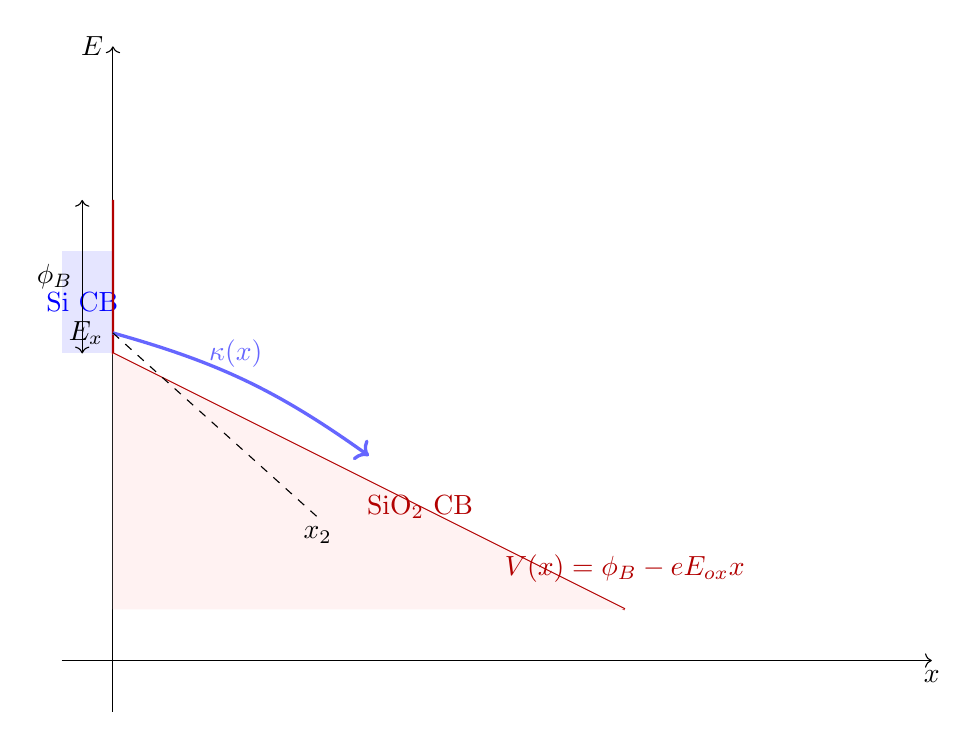
\begin{tikzpicture}[scale=1.3]
  % Energy axis
  \draw[->] (0,-0.5) -- (0,6) node[left] {$E$};
  \draw[->] (-0.5,0) -- (8,0) node[below] {$x$};
  % Si conduction band
  \fill[blue!10] (-0.5,3) rectangle (0,4);
  \node[blue] at (-0.3,3.5) {Si CB};
  % SiO2 barrier
  \draw[thick, red!70!black] (0,4.5) -- (0,3) -- (5,0.5);
  \fill[red!5] (0,0.5) -- (0,3) -- (5,0.5) -- (5,0.5) -- (0,0.5);
  \node[red!70!black] at (3,1.5) {SiO$_2$ CB};
  % Barrier height
  \draw[<->] (-0.3,3) -- (-0.3,4.5) node[midway,left] {$\phi_B$};
  % Tunneling arrow
  \draw[->,very thick,blue!60] (0,3.2) to [bend left=10] (2.5,2.0);
  \node[blue!60] at (1.2,3.0) {$\kappa(x)$};
  % E_ox
  \node[red!70!black] at (5,0.9) {$V(x) = \phi_B - eE_{ox}x$};
  % Turning points
  \draw[dashed] (0,3.2) -- (0,3.2) node[left] {$E_x$};
  \draw[dashed] (0,3.2) -- (2.0,1.4) node[below] {$x_2$};
\end{tikzpicture}
\caption{Fowler-Nordheim隧穿的能带图。当氧化层电场 $E_{ox}$ 倾斜SiO$_2$导带
成为三角形势垒时，电子从Si导带（左）隧穿通过势垒。
WKB近似将该三角形势垒的隧穿概率严格积分化。}
\label{fig:fn-barrier}
\end{figure}

\begin{physbox}
  \textbf{FN电流的极致非线性。}在编程电场 $E_{ox} \approx \SI{1.0e9}{V/m}$ 下，
  $J_{FN} \sim \SI{1e4}{A/cm^2}$（编程时间 \SI{100}{\mu s}）。
  零偏压下（$E_{ox} \approx 0$），$J_{FN} \to 0$（严格为 $< 10^{-20}$ A/cm$^2$）。
  编程态与非偏态之间的电流比值 $\sim 10^{20}$——这解释了为何FN隧穿能同时满足
  \SI{100}{\mu s} 编程和 \SI{10}{year} 数据保持的两个极端要求。
  这一\"开关比\"是任何基于热激活机制的存储技术（如PCM）无法企及的。
\end{physbox}

\subsection{编程操作的物理：ISPP收敛性分析}

编程操作的控制栅加高压 $V_{CG} \approx \SI{15}{-20}{V}$，
源/漏/衬底接地。隧穿氧化层上的电压 $V_{ox} \approx \alpha_{CG} V_{CG}$，
产生 $E_{ox} \approx \SIrange{0.8}{1.5e9}{V/m}$。
电子从沟道FN隧穿进入浮栅，浮栅电位随之下降，
减小 $V_{ox}$——这是一个\textbf{自限充电过程}。

虽然从第一性原理可以推导 $V_{FG}(t)$ 的解析渐近式，但在实际器件中，
为了精确控制编程后的阈值分布，采用的不是单一大脉冲而是
\textbf{增量步进脉冲编程（ISPP）}：

\begin{enumerate}
  \item 施加编程脉冲（宽度 $t_p \approx \SI{10}{-30}{\mu s}$，幅度 $V_{PGM}$）。
  \item 执行编程验证读取，判断 $V_{th}$ 是否超过目标值 $V_{th}^{\text{target}}$。
  \item 若未达到，增加 $V_{PGM} \leftarrow V_{PGM} + \Delta V_{PGM}$
  （步长 $\Delta V_{PGM} \approx \SI{0.2}{-0.5}{V}$），返回步骤1。
  \item 已达到目标 → 该单元标记为\"编程禁止\"（通过自举偏置将沟道电位抬高，
  减小 $V_{ox}$）。
\end{enumerate}

ISPP的收敛性：每步阈值电压的增量近似为 $\Delta V_{th} \approx \alpha_{CG} \cdot \Delta V_{PGM}$。
第 $k$ 步后 $V_{th}$ 分布的标准差 $\sigma_{V_{th}} \approx \alpha_{CG} \cdot \Delta V_{PGM} / 2$
（假设初始分布宽度可忽略）。
因此减小 $\Delta V_{PGM}$ 可缩小编程分布——但代价是编程步数增加（延长写入时间）。
这是MLC/TLC设计中的核心权衡。

\subsection{直接隧穿与保持时间}

当氧化层厚度 $t_{ox} < \SI{3}{nm}$ 时，即使在零电场下，
电子也可通过\textbf{直接量子隧穿（Direct Tunneling, DT）}穿过
梯形势垒（\cref{fig:dt-barrier}）。DT概率近似为：
\begin{equation}
  T_{DT} \approx \exp\!\left( -\frac{2\sqrt{2m^*_{ox}}}{\hbar}
            \sqrt{\phi_B}\, t_{ox} \right)
\end{equation}

当前NAND闪存的 $t_{ox} \approx \SI{5}{-7}{nm}$ 是编程速度与数据保持之间的最优权衡点：
在此厚度下DT概率在零偏压下可忽略（保持时间 >\SI{10}{yr}），
但在高电场下FN隧穿电流充足（编程时间 <\SI{100}{\mu s}）。

% ===================================================================
\section{多级存储的物理极限}
\label{sec:mlc}

\subsection{阈值电压窗口的划分与分布模型}

在总阈值窗口 $\Delta V_{th}^{\text{total}} \approx \SI{4}{V}$ 内
（从擦除态 \SI{\sim 0.5}{V} 到最高编程态 \SI{\sim 4.5}{V}），
$2^n$ 个状态被分配在优化间距的电压上。
第 $k$ 个状态的阈值电压分布近似高斯：
\begin{equation}\label{eq:vth-gauss}
  p_k(V) = \frac{1}{\sqrt{2\pi}\,\sigma_k}
           \exp\!\left[ -\frac{(V - \mu_k)^2}{2\sigma_k^2} \right]
\end{equation}
其中 $\mu_k$ 为中心值，$\sigma_k$ 为标准差。

由于编程过程中浮栅电荷的统计涨落（电子注入的Poisson性、CCI的随机性、RTN等），
$\sigma_k$ 通常随状态编号 $k$ 增大而增加——即高 $V_{th}$ 态的分布更宽。
典型TLC的 $\sigma$ 范围为 \SI{40}{-80}{mV}，
QLC可低至 \SI{30}{-50}{mV}（需更严密的编程算法）。

\subsection{相邻状态的判决阈值与原始误码率}

相邻状态 $k$ 与 $k+1$ 间的最优判决阈值 $V_{opt}$ 由最大后验（MAP）准则给出。
假设等先验概率，$V_{opt}$ 由似然比方程 $p_k(V_{opt}) = p_{k+1}(V_{opt})$ 确定。
当 $\sigma_k = \sigma_{k+1} = \sigma$ 时简化为中点
$V_{opt} = (\mu_k + \mu_{k+1}) / 2$。

原始位错误率（Raw BER）由Gauss尾部的交叠积分给出：
\begin{equation}\label{eq:raw-ber}
  \boxed{ \text{BER}_{\text{raw}}
  = \frac{1}{2}\,\operatorname{erfc}\!\left(
    \frac{\Delta V}{2\sqrt{2}\,\sigma}
  \right) }
\end{equation}
其中 $\Delta V = \mu_{k+1} - \mu_k$ 为级间距，
互补误差函数 $\operatorname{erfc}(x) = (2/\sqrt{\pi}) \int_x^\infty e^{-t^2} dt$。

\begin{physbox}
  \textbf{TLC BER的数值示例。}取 $\Delta V = \SI{400}{mV}$，
  $\sigma = \SI{60}{mV}$，
  则 $\Delta V/(2\sqrt{2}\sigma) \approx 2.357$，
  $\operatorname{erfc}(2.357) \approx 8.5 \times 10^{-4}$。
  $\text{BER}_{\text{raw}} \approx \num{4.2e-4}$——
  这意味着约每 2400 bit 就有 1 bit 是错的。

  这必须通过LDPC或BCH纠错码校正至 $< 10^{-15}$。
  编码开销（code rate）约为 $0.85$--$0.93$，
  意味着 \SI{15}{\%}{--}\SI{7}{\%} 的闪存容量被ECC冗余占用。
\end{physbox}

\subsection{电子数的Poisson涨落：QLC的根本物理限制}

对于QLC（16级），级间距仅 \SI{150}{-250}{mV}。
每个状态下浮栅中的电子数 $\bar{N} \approx C_{IPD} (\mu_k - V_{th0}) / e$。
对于最小编程态，$\bar{N} \approx 50$--$100$。
Poisson涨落 $\sigma_N = \sqrt{\bar{N}} \approx 7$--$10$ 个电子。
对应的 $\sigma_{V_{th}} \approx \sigma_N \times e / C_{IPD}
\approx \SI{60}{-130}{mV}$。

将电子数的Poisson贡献、CCI贡献和RTN贡献平方相加，总 $\sigma_{V_{th}}$ 可能达到
\SI{80}{-150}{mV}——与级间距可比。这是QLC存储\"可行但边缘\"的物理原因。
进一步增加每单元比特数（PLC, 5 bits/cell, 32级）需要在有限的总窗口内挤出
\SI{<100}{mV} 的间距，Poisson噪声使其在现有浮栅技术下不可行——
除非采用不同的物理机制（如铁电、相变等全新器件）。

% ===================================================================
\section{隧穿氧化层的退化与可靠性物理}
\label{sec:degradation}

\subsection{应力诱导漏电流（SILC）的陷阱辅助模型}

每次擦写循环中，FN隧穿的高能电子（能量可达 \SI{5}{-8}{eV}）会打断Si--O键，
产生氧化层体陷阱和Si/SiO$_2$界面态。主要微观机制：

\begin{itemize}
  \item \textbf{Si--H键断裂}：在沟道界面处，钝化Si--H键被高能电子打断，
  产生Si悬挂键（$P_b$中心，即三配位Si$\bullet$）。
  释放的H原子可扩散至氧化层内部，H$^+$在电场下漂移形成空间电荷。
  \item \textbf{氧空位生成}：SiO$_2$网格中的O原子受高能电子撞击移位，
  产生氧空位 $E'$ 中心（$\equiv \text{Si}\bullet\,\text{Si}\equiv$）。
\end{itemize}

陷阱产生率与注入电荷总量 $Q_{inj}$ 的幂律关系：
$\Delta N_{it} \propto Q_{inj}^n$，
指数 $n \approx 0.4$--$0.6$（取决于氧化层工艺。干氧 > 湿氧）。

陷阱辅助隧穿（Trap-Assisted Tunneling, TAT）：氧化层中的缺陷能级充当
\"跳板\"，使电子分步隧穿——等效降低了势垒厚度（\cref{fig:tat}）：
\begin{equation}\label{eq:tat}
  J_{TAT} \propto N_{trap} \exp\!\left(
    -\frac{8\pi\sqrt{2m_{ox}^*}}{3h E_{ox}} \phi_t^{3/2}
  \right)
\end{equation}
其中 $\phi_t$ 为陷阱的能级深度（从SiO$_2$导带测量）。

\begin{figure}[H]
\centering
\begin{tikzpicture}[scale=1.2]
  \draw[->] (0,-0.5) -- (0,6) node[left] {$E$};
  \draw[->] (-0.5,0) -- (8,0) node[below] {$x$};
  \draw[thick,red!70!black] (0,4.5) -- (0,3) -- (7,0);
  % Traps
  \filldraw (1.5,3.2) circle (2pt) node[above] {$E_t$};
  \filldraw (3.0,2.5) circle (2pt) node[above] {$E_t$};
  \filldraw (4.5,1.8) circle (2pt) node[above] {$E_t$};
  % Tunneling hops
  \draw[->,blue!60,very thick] (0,3.2) -- (1.5,3.2);
  \draw[->,blue!60,very thick] (1.5,3.2) -- (3.0,2.5);
  \draw[->,blue!60,very thick] (3.0,2.5) -- (4.5,1.8);
  \draw[->,blue!60,very thick] (4.5,1.8) -- (6.5,0.5);
  \node[blue!60] at (7.5,1.5) {TAT路径};
  % FN for comparison
  \draw[->,gray,dashed] (0,3.5) to [bend left=10] (5,0);
  \node[gray] at (6,3) {FN路径};
\end{tikzpicture}
\caption{陷阱辅助隧穿（TAT）的示意。氧化层中的缺陷能级（$E_t$）提供中间态，
电子分多步隧穿——等效势垒高度从 $\phi_B$ 降低到 $\phi_t$。
随着P/E循环增加，陷阱密度 $N_{trap}$ 升高，TAT电流增大，
加速数据保持失效。}
\label{fig:tat}
\end{figure}

\subsection{随机电报噪声（RTN）}

当单个氧化层陷阱恰好位于沟道界面附近时，该陷阱对电子的捕获/释放随机切换
（Poisson过程），导致 $V_{th}$ 在离散的两个水平间跳变——即\textbf{随机电报噪声（RTN）}。
RTN导致的 $V_{th}$ 跳变幅度约为：
\begin{equation}
  \Delta V_{th}^{RTN} \approx \frac{e}{W L C_{ox}}
\end{equation}
对于 $W \times L = \SI{20}{nm} \times \SI{20}{nm}$ 的单元，
$C_{ox} \approx \SI{2.5e-17}{F}$，
$\Delta V_{th}^{RTN} \approx \SI{6}{mV}$——听起来小，但对于QLC
（级间距 \SI{150}{mV}），$6\sigma$ 噪声预算已相当紧张。

更严重的是，RTN的\textbf{低频功率谱密度}为 $1/f$ 型，
意味着长时间观测会引入更大的 $V_{th}$ 摆动。读取判决时刻若恰逢RTN的\"坏相位\"，
可导致单次读取错误。

\subsection{Arrhenius数据保持与温度加速}

数据保持时间的温度依赖性：
\begin{equation}\label{eq:arrhenius}
  t_{\text{ret}}(T) = t_{\text{ret}}(T_0)
  \exp\!\left[ \frac{E_a}{k_B}
            \left( \frac{1}{T} - \frac{1}{T_0} \right) \right]
\end{equation}
其中激活能 $E_a \approx \SI{1.0}{-1.2}{eV}$
（对应电子从SiO$_2$深陷阱热发射越过Si/SiO$_2$界面势垒）。

在室温（\SI{300}{K}）附近，$E_a/k_B \approx \SI{1.16e4}{K}$，
这意味着：温度每升高约 \SI{5}{\degC{}}，保持时间约减半
（$t_{\text{ret}}(\SI{305}{K}) \approx 0.5 \times t_{\text{ret}}(\SI{300}{K})$）。

这是SSD工作温度规范（通常上限 \SI{70}{\degC{}}）的根本物理原因——
当SSD在数据中心高温环境下以无主动散热方式运行时，
数据保持时间可能从 \SI{10}{yr} 降至 \SI{1}{-2}{yr}。
这也是\"冷存储\"（cold storage，\SI{25}{\degC{}}）比
\"温热存储\"能显著延长SSD存档寿命的原因。

% ===================================================================
\section{NAND阵列组织与闪存转换层}
\label{sec:array}

\subsection{NAND串的电学模型}

NAND闪存的基本单元是\textbf{串（String）}：32--128个浮栅晶体管串联，
两端通过选择晶体管（SSL, DSL）连接到位线（BL）和源线（SL）。
串联架构的物理后果：

\begin{itemize}
  \item \textbf{读取电阻}：被选中单元的导通电阻与所有未选中单元
  （被 $V_{pass} \approx \SI{5}{-6}{V}$ 强制导通在线性区）
  的沟道电阻串联。单个单元的沟道电阻约 \SI{10}{k\Omega}，
  128个串联时 $\sim \SI{1.3}{M\Omega}$。
  读取电流约 \SI{\sim 1}{\mu A}（$V_{BL} \approx \SI{1}{V}$）。
  \item \textbf{自举效应（Self-Boosting）}：当某单元被禁止编程时，
  其沟道通过未选中字线的高压（$V_{pass}$）电容耦合抬高，
  减小隧穿氧化层上的 $V_{ox}$，从而抑制寄生FN隧穿。
  自举效率取决于沟道与字线间的电容耦合比。
\end{itemize}

\subsection{块擦除的物理必然性}

NAND闪存的擦除以\textbf{块（Block）}为单位（通常 64--512 页，
每页 \SI{16}{KB}）。物理原因：
所有单元的p阱（body）共享同一衬底接触，擦除时需对整个p阱加高压
$V_{ERS} \approx \SI{15}{-20}{V}$（控制栅接地），
无法仅对单个单元施加擦除条件。

这一事实直接推导出NAND闪存的\textbf{核心物理限制：不能原地覆写}。
任何\"修改页数据\"的操作在物理上只能是：
\begin{enumerate}
  \item 在新物理页写入修改后的数据。
  \item 将旧页标记为逻辑无效（stale）。
  \item 当整个块的无效页占比足够高时，GC回收该块（复制有效页 $\to$ 擦除整个块）。
\end{enumerate}

\subsection{闪存转换层（FTL）与数据残留}

FTL维护逻辑块地址（LBA）到物理页地址（PPA）的动态映射。
当主机覆写LBA $X$ 时：
\begin{itemize}
  \item FTL分配新物理页 $P_{\text{new}}$，写入新数据。
  \item 原物理页 $P_{\text{old}}$ 标记为无效（stale）。
  \item $P_{\text{old}}$ 中的浮栅电荷\textbf{完好无损}——电子安稳地存储在浮栅中，
  直到该块被GC回收并执行物理擦除（FN隧穿移除所有浮栅电荷）。
\end{itemize}

\textbf{物理后果}：从写入数据到GC物理擦除之间存在不可预测的时间窗口
（可长达数周甚至永不，若SSD从未满）。在此期间，逻辑上\"已删除\"的数据
以完整的物理形式残留在闪存中——这正是固态存储数据恢复的物理基础
（详见第5篇《数据删除与恢复的物理原理》）。

\subsection{3D NAND：从浮栅到电荷陷阱}

2013年后，NAND从平面转向垂直堆叠（3D NAND），当前超过300层。
关键的物理转变是用\textbf{电荷陷阱氮化硅（Si$_3$N$_4$）}
替代多晶硅浮栅作为电荷存储介质。

Si$_3$N$_4$中电荷被离散的深能级陷阱捕获（陷阱密度 $\sim 10^{19}$ cm$^{-3}$，
能级深度 $\sim \SI{1.0}{-1.5}{eV}$），而非均匀分布在浮栅中。
优势：
\begin{itemize}
  \item 电荷局域化——CCI大幅降低。
  \item 更薄的存储层（$\sim \SI{5}{nm}$ vs $\sim \SI{10}{nm}$浮栅），适合垂直堆叠。
  \item 陷阱间互相隔离——单个陷阱的泄漏不影响邻近陷阱。
\end{itemize}

3D NAND采用\"栅极优先\"（gate-first）或\"替换栅\"（replacement gate）工艺，
字线为水平钨（W）层，沟道为垂直多晶硅柱（macaroni结构）。
电荷捕获层的编程机制仍是FN隧穿，但电荷注入Si$_3$N$_4$层后，
通过\textbf{Poole-Frenkel发射}在陷阱间跃迁分布。

% ===================================================================
\section{结论与展望}
\label{sec:conclusion}

NAND闪存的物理基础可归纳为以下核心框架：

\begin{enumerate}
  \item \textbf{电容耦合模型}：$V_{th} = V_{th0} + Q_{FG}/C_{IPD}$——
  阈值电压是浮栅电荷的线性函数，斜率为 $1/C_{IPD} \sim \SI{0.1}{V/e}$。

  \item \textbf{FN隧穿}：$J = A E_{ox}^2 \exp(-B/E_{ox})$——
  电流对电场的超指数敏感性，解释了 \SI{100}{\mu s} 编程与 \SI{10}{yr} 保持
  如何能共存于同一器件。

  \item \textbf{多级存储极限}：判决误码率
  $\text{BER} = (1/2)\operatorname{erfc}(\Delta V/(2\sqrt{2}\sigma))$，
  由阈值分布的交叠积分决定。底层受电子Poisson涨落约束——
  $\sigma_N = \sqrt{\bar{N}}$ 使QLC处于\"可行但边缘\"的物理域。

  \item \textbf{退化}：氧化层陷阱积累 $\to$ SILC + TAT + RTN
  $\to$ 保持时间缩短 $\to$ P/E寿命终了。
  Arrhenius定律 $t_{\text{ret}} \propto \exp(E_a/k_B T)$
  解释了高温下的加速失效。

  \item \textbf{FTL与数据残留}：异地更新策略使逻辑删除后的物理数据长期残留。
  GC的不可预测延迟是数据恢复的根本窗口。
\end{enumerate}

NAND闪存的未来方向包括：400+层3D堆叠、铁电FET（FeFET）替代电荷陷阱、
存内计算架构。但浮栅/电荷陷阱的物理机制作为当前非易失性半导体存储的基础，
其深层理解——从FN的WKB推导到Poisson电子数涨落——
仍然是设计、优化和可靠使用闪存的前提。

% ===================================================================
\appendix
\section{关键物理参数}

\begin{table}[H]
\centering
\caption{NAND闪存涉及的关键物理参数}
\begin{tabular}{@{}llll@{}}
\toprule
参数 & 符号 & 典型值 & 单位 \\
\midrule
隧穿氧化层厚度 & $t_{tun}$ & 5--7 & nm \\
SiO$_2$/Si势垒高度 & $\phi_B$ & 3.15 & eV \\
SiO$_2$电子有效质量 & $m_{ox}^*$ & 0.42 & $m_e$ \\
IPD等效氧化层厚度 & $t_{IPD}$ & 10--20 & nm \\
编程电压 & $V_{PGM}$ & 15--20 & V \\
擦除电压 & $V_{ERS}$ & 15--20 & V \\
ISPP步长 & $\Delta V_{PGM}$ & 0.2--0.5 & V \\
控制栅耦合比 & $\alpha_{CG}$ & 0.50--0.65 & — \\
单电子阈值偏移 & $\Delta V_{th}^{1e}$ & $\sim 100$--150 & mV \\
数据保持激活能 & $E_a$ & 1.0--1.2 & eV \\
TLC P/E寿命 & — & $1\times 10^3$--$3\times 10^3$ & 次 \\
QLC P/E寿命 & — & $5\times 10^2$--$1\times 10^3$ & 次 \\
\bottomrule
\end{tabular}
\end{table}

% ===================================================================
\begin{thebibliography}{99}

\bibitem{sze}
S. M. Sze and K. K. Ng, \textit{Physics of Semiconductor Devices}, 3rd ed.
Wiley, 2007.
\href{https://doi.org/10.1002/0470068329}{doi:10.1002/0470068329}

\bibitem{bez}
R. Bez, E. Camerlenghi, and A. Modelli,
``Introduction to flash memory,''
\textit{Proc. IEEE}, vol. 91, no. 4, pp. 489--502, 2003.
\href{https://doi.org/10.1109/JPROC.2003.811702}{doi:10.1109/JPROC.2003.811702}

\bibitem{lenzlinger}
M. Lenzlinger and E. H. Snow,
``Fowler--Nordheim tunneling into thermally grown SiO$_2$,''
\textit{J. Appl. Phys.}, vol. 40, pp. 278--283, 1969.
\href{https://doi.org/10.1063/1.1657811}{doi:10.1063/1.1657811}

\bibitem{prall}
K. Prall,
``Scaling non-volatile memory below 30nm,''
\textit{IEEE Non-Volatile Semiconductor Memory Workshop}, pp. 5--10, 2007.
\href{https://scholar.google.com/scholar?q=Prall+scaling+non-volatile+memory+below+30nm}{Google Scholar}

\bibitem{cai}
Y. Cai, E. F. Haratsch, O. Mutlu, and K. Mai,
``Error patterns in MLC NAND flash memory: Measurement, characterization, and analysis,''
\textit{Proc. DATE}, pp. 521--526, 2012.
\href{https://doi.org/10.1109/DATE.2012.6176524}{doi:10.1109/DATE.2012.6176524}

\bibitem{micheloni}
R. Micheloni and L. Crippa,
\textit{Inside NAND Flash Memories}.
Springer, 2010.
\href{https://doi.org/10.1007/978-90-481-9431-5}{doi:10.1007/978-90-481-9431-5}

\bibitem{mielke}
N. Mielke, T. Marquart, N. Wu, J. Kessenich, H. Belgal, E. Schares, F. Trivedi, E. Goodness, and L. R. Nevill,
``Bit error rate in NAND Flash memories,''
\textit{IEEE IRPS}, pp. 9--19, 2008.
\href{https://doi.org/10.1109/RELPHY.2008.4558857}{doi:10.1109/RELPHY.2008.4558857}

\bibitem{cappelletti}
P. Cappelletti, C. Golla, P. Olivo, and E. Zanoni (eds.),
\textit{Flash Memories}.
Kluwer Academic Publishers, 1999.
\href{https://doi.org/10.1007/978-1-4615-5015-0}{doi:10.1007/978-1-4615-5015-0}

\end{thebibliography}

\end{document}
